 \documentclass{beamer}
\beamertemplatenavigationsymbolsempty
\usepackage{amsmath, amssymb, hyperref, graphics, tikz}
\usepackage[normalem]{ulem} %for strikeout \sout{ }



\newcommand{\C}{\mathbb{C}}
\newcommand{\Z}{\mathbb{Z}}
\newcommand{\R}{\mathbb{R}}
\newcommand{\N}{\mathbb{N}}
\DeclareMathOperator{\Real}{Re}
\DeclareMathOperator{\Imag}{Im}


\begin{document}
\begin{frame}{Consequences of Cauchy's Theorem}
    
\begin{theorem}[Cauchy's Theorem] Suppose the function $f$ is analytic on a \alert{simply connected} region $D$.  Then $\int_\gamma fdz=0$ for \emph{all} contours $\gamma$ in $D$.
\end{theorem}

\begin{corollary}[Independence of Path]
Let $f$ be analytic on a simply-connected region $D$ and let $\gamma_1$ and $\gamma_2$ be any two paths in $D$ from $a$ to $b$. Then:
 $$\int_{\gamma_1}f(z)dz=\int_{\gamma_2}f(z)dz$$
\end{corollary}
\begin{proof} If we do $\gamma_1$ then $\gamma_2$ backwards, we get a contour, and can apply Cauchy.
\end{proof}
\end{frame}
\begin{frame}{Applications of path independence}
\begin{example}[8.4]Let $\gamma$ be any path from $-i$ to $i$ that cross $\R$ only between -1 and 1.  Evaluate $\int_\gamma\frac{dz}{1-z^2}$.
\end{example}
\begin{block}{Cauchy and ML: two great tastes that taste great together}
\begin{example}[8.5]
Let $\alpha$ be any path in $D=\{z\in\C : |z|<2\}$.  Find $B$ so that
$$\left|\int_\alpha \frac{\sinh(z)}{9+e^z}dz\right|\leq B.$$
\end{example}

\end{block}

\end{frame}

\begin{frame}{Application of Cauchy's Theorem: existence of primitives}
I claimed that whenever Cauchy's Theorem applied, $f$ has a primitive.  More precisely:
\begin{lemma}
Let $D$ be a simply connected domain, and let $f$ be analytic on $D$.  Let $p\in D$ be any point, and define a function $F$ on $D$ by $F(z)=\int_\alpha f(z)dz$ where $\alpha$ is any path in $D$ from $p$ to $z$.  Then for any path $\gamma:[a,b]\to D$ we have
$$\int_\gamma f(z)dz = F(\gamma(b))-F(\gamma(a))$$
Furthermore, $F$ is analytic on $D$, and $F^\prime=f.$
\end{lemma}



\end{frame}


\begin{frame}{Too many memes are sexist/heteronormative.  Sorry.}
\begin{columns}
\begin{column}{0.6\textwidth}
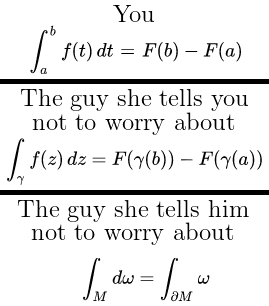
\includegraphics[width=\textwidth,height=0.8\textheight,keepaspectratio]{WorryAboutStokes.png}
\end{column}
\begin{column}{0.4\textwidth}  %%<--- here

The last formula is Stoke's Theorem, which generalizes Green's theorem to higher dimensions.

\end{column}
\end{columns}

\end{frame}

\begin{frame}{Section 9: Cauchy's Integral Formula and Consequences}
\begin{theorem}[Cauchy's integral formula] Let $\gamma$ be a simple contour described in the positive direction.  Let $w$ lie inside $\gamma$.  Suppose that $f$ is analytic on a simply connected region $D$ containing $\gamma$ and its interior.  Then:

$$f(w)=\frac{1}{2\pi i} \int_\gamma\frac{f(z)}{z-w}dz.$$

\end{theorem}
\begin{block}{Sketch of proof}
\begin{enumerate}
    \item Theorem 9.1 ``Deforming contours'': replace $\gamma$ with $w+\varepsilon e^{2\pi i t}$ and take $\varepsilon\to 0$
    \item  $$????\quad\frac{f(z)-f(w)}{z-w}\quad????$$
    \item \sout{Profit} Prove the Theorem
\end{enumerate}
\end{block}

\end{frame}
\begin{frame}{Theorem 9.1 Deforming Contours}
\begin{theorem} Let $\gamma$ be a simple contour described in the positive direction.  Let $z_0$ be a point inside $\gamma$, and let $C$ be another simple contour in positive direction, contained entirely inside $\gamma$. Suppose that $f$ is analytic on a region $D$ which contains $\gamma, C$ and all points in between.  Then
$$\int_\gamma f(z)dz=\int_C f(z)dz$$
\end{theorem}
\begin{itemize}
    \item Crucially, $D$ need \alert{not} be simply connected
    \item Proof: join $C$ and $\gamma$ together by two paths, and rearrange contours to apply Cauchy.
\end{itemize}


\end{frame}
\end{document}
